%
%  untitled
%
%  Created by Sam Anzaroot on 2012-10-05.
%  Copyright (c) 2012 __MyCompanyName__. All rights reserved.
%
\documentclass[twocolumn,letterpaper]{article}

% Use utf-8 encoding for foreign characters
\usepackage[utf8]{inputenc}

% Setup for fullpage use
\usepackage{fullpage}

% Multipart figures
%\usepackage{subfigure}

% More symbols
\usepackage{amsmath}

% Package for including code in the document
\usepackage{listings}

\usepackage{ifpdf}

\ifpdf
\usepackage[pdftex]{graphicx}
\else
\usepackage{graphicx}
\fi

\usepackage{todonotes}

\setlength{\marginparwidth}{2cm}

\title{Author Linkage in Records using Temporal Information and Conditional Random Fields : A midterm report}
\author{Sam Anzaroot, Jiaping Zheng}

\date{}

\begin{document}

\ifpdf
\DeclareGraphicsExtensions{.pdf, .jpg, .tif}
\else
\DeclareGraphicsExtensions{.eps, .jpg}
\fi

\maketitle

\section{Introduction} % (fold)
\label{sec:introduction}
Record Linking is the task of clustering records in a database such that elements in the same cluster refer to the same real world object. For example, in the DBLP page for David Smith, there are at least three different individuals with publications named David Smith appearing, and the output of a record linker would cluster each David Smith's publications into separate clusters. Various attempts have been made for record linking authors of publications listed in datasets such as DBLP. This task is important because there are many downstream applications that require clean clustering of such information, for example, determining the most prolific authors is only accurate if such clusterings are valid. Network analysis of coauthorship also depends on correct clustering of authors. In this report, we define strings of author names as author mentions, and clusters of author mentions referring to the same person as entities. The goal of the task is to cluster all mentions into the appropriate entities. This task requires a classifier to determine the matchings between two mentions. This task is not a solved one, and we will attempt to build a more robust classifier.
% section introduction (end)

\section{Related Work} % (fold)
\label{sec:related_work}
\paragraph{Survey of Related work} % (fold)
\label{par:survey_of_related_work}
The research field of record clustering is a very active one. This task is important for many different applications, and as such there are many different names for this task, including record clustering, record deduplication, record linking, entity resolution, etc. There are many components to a record linking system. The first are methods of paring down which records are in need of clustering for efficiency, called blocking methods. The task also requires a system for classifying whether or not a set of records match. In addition, methods of effectively clustering supersets of records independently classified are necessary. In order to classify records, effective similarity and/or compatibility measures are needed as features in a classifier. In this report, we are focusing in on building a better classifier for disambiguating authors in DBLP, and generating better features.
% paragraph survey_of_related_work (end)

Similarity metrics are important for classification as they provide information in which a classifier can make a decision on. Others have shown that adding temporal information into metrics can enhance the quality of classification \cite{DBLP:journals/fcsc/LiDMS12}. These metrics are weighted by how relevant the metrics are given the distance in time between the two records. This weighting is learned from a set of annotated data.

Various numbers of people have attempted to build classifiers using graphical models that include complex dependencies. For example, ``Multi-Relational Record Linkage'' \cite{Domingos04multi} models the record linking problem as a conditional random field which improved F1 performance on a publication deduplication task. In this CRF model, each pair of publication records has a binary latent variable to model whether the records are duplicates.  The observations are modeled using similarity functions.  ``Information nodes'' connect the binary duplication variables and the observation nodes which represent whether the fields of the publication in two records match.

``A Conditional Model of Deduplication for Multi-Type Relational Data'' \cite{Culotta05aconditional} extends the model previously stated by making the ``information nodes'' first-class variables in the model.  Binary latent variables that indicate record duplication (both paper and venue) are connected in the CRF to capture the interdependencies between the deduplication results of publications and venues.  For example, equivalent venue records that are merged should result in weights in CRF that also encourage merging of paper records.  To perform inference of finding optimal configurations of the latent variables, the authors convert the model into a weighted undirected graph to find a optimal partitioning.  Learning is approximated by maximizing the product of local marginals using limited-memory BFGS.  Their experiments show an up to a 30\% error reduction in venue deduplication and 20\% in paper deduplication.
% section related_work (end)

\section{Methodology} % (fold)
\label{sec:methodology}
We model the author linkage problem in a conditional random field.

Conditional random fields (CRFs) are undirected graphical models that encode the conditional probability of a set of unobserved random variables $Y$ given a set of observed variables $X$.  Usually the probability can be factored using independence assumptions.  The model can be represented in a graph $G$, where the vertices correspond to the variables $X$ and $Y$.  A potential function $\phi_c$ is defined for every clique $c$ in the graph.  The conditional probability $p(y|x)$ can be expressed as
$$p(y|x)=\frac{1}{Z}\prod_c \phi_c(x_c,y_c),$$
where $Z=\sum_y\prod_c \phi_c(x_c,y_c)$ is a normalization factor.  We assume $\phi_c$ is a log-linear combination of feature functions of the variables in clique $c$, thus
$$\phi_c(x_c,y_c)=\exp\left(\sum_k \lambda_k f_k(x_c,y_c)\right).$$

The model parameters $\{\lambda_k\}$ are learned from training data by
maximum likelihood estimation.  In a CRF model, the log likelihood
function is optimized using numerical optimization methods, such as
limited-memory BFGS or conjugate gradient method.

Inference corresponds to finding the optimal assignments to the $Y$
variables such that $p(y|x)$ is maximized.  Belief propagation is an
exact inference algorithm on tree-structured models.  Approximate
algorithms on models with cycles include loopy belief propagation and
MCMC methods.



Specifically, our CRF structure models the conditional probability of
two author mentions referring to the same entity given the publication
information.  The unobserved random variables in our model include one
binary variable for each pair of author mentions that indicates
whether they refer to the same person.  We also define latent random
variables that represent the compatibility between the names of the
authors, between the publication venues, between their affiliations,
and between their coauthors.  The observed variables are similarity
features between author names, venues, affiliations, and coauthors.
The model is shown in Figure \ref{fig:crf}.

\begin{figure*}
\centering
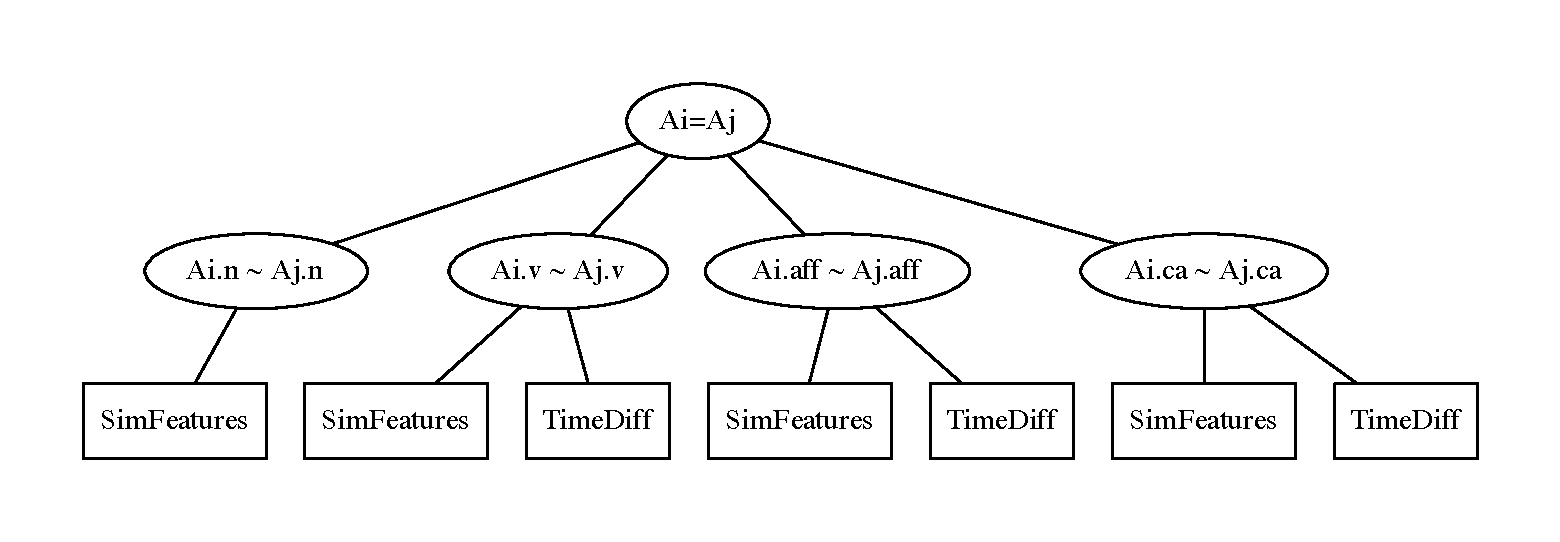
\includegraphics[width=\textwidth]{crf}
\caption{Our CRF model for the author linkage problem.  $A_i$ denotes
  the $i$th author string.  $A_i.n$, $A_i.v$, $A_i.aff$, and $A_i.ca$
  denote the name, venue, affiliation, and coauthors of $A_i$.  The
  oval nodes are unobserved random variables, and the box-shaped ones
  are observed variables.}
\label{fig:crf}
\end{figure*}

\begin{figure}
\centering
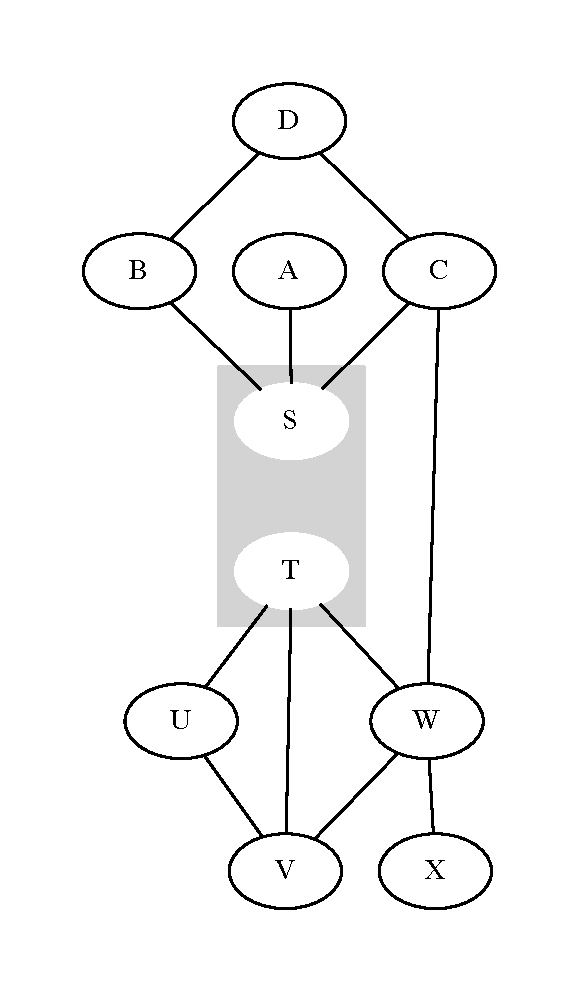
\includegraphics[height=.32\textheight]{coauthor}
\caption{A coauthorship network.  The nodes represent author strings
  in the database.  An edge between two nodes means that the two
  authors coauthored a paper.  $S$ and $T$ are the two author mentions
  that the model is classifying. Edges between $S$, $T$ and other
  nodes mean that the other node is a coauthor mention in the
  publication containing the mentions $S$ and $T$.}
\label{fig:coauthor}
\end{figure}

Unlike the model proposed in Culotta and McCallum
\cite{Culotta05aconditional}, which deduplicates publication title and
venues jointly, our model focuses on author coreference resolution.
Learning and inference in such a complicated model is intractable.
However, since the DBLP data is generated directly from entire
conference proceedings and journals, the publication records are less
noisy.  Our model takes advantage of the reliability of the source
data and deduplicates only ambiguous author information.  Therefore,
our model is more scalable.

Linking pairs of author names is only the first step in the author
linkage problem.  To generate clusters of author mentions that refer
to the same person, we take the transitive closure of the pairwise
predictions from the CRF model.

Since we are comparing pairs of author mentions, it's impractical to
consider all the $O(n^2)$ pairs in the dataset.  We'll also be wasting
effort because most of the pairs clearly do not refer to the same
author.  We follow the method in \cite{McCallum00} to first cluster
the author strings into ``canopies'' and only compare pairs within the
same canopy.  Canopies are soft clusters that can have overlapping
author mentions.  This approach can significantly reduce the number of
pairs we need to compare, and the soft nature of the clusters help
mitigate the problem that the clustering algorithm may have
inaccurately partitioned the data set.


\paragraph{Similarity Features} % (fold)
\label{par:similarity_features}
In order to perform classification we will make use of various similarity and compatibility metrics. One useful metric is string similarity. Simple Levenstein edit distance often works poorly in many of the applications in this domain such as name comparison, since names are often represented in different formats, with the ordering switched, abbreviated etc. Hybrid methods, which combine string-edit distance with token based methods, often are the best performing distance metric in similar tasks \cite{cohen2003comparison}. One such metric is SoftTFIDF. SoftTFIDF works like TFIDF, but on similar tokens instead of just matching tokens. It uses the Jaro-Winkler metric as the similarity metric for tokens. 

The Jaro similarity metric for $s$ and $t$ given $s= s_1,s_2,s_3...$ and $t= t_1,t_2,t_3...$ defines a match of $s_i$ to a character $t_j$ if $s_i=t_j$ and j is $\frac{min(s,t)}{2} < |i-j|$. Define $s'$ as the characters that match in $s$ and $t'$ are the characters that match in t. Additionaly, define $T$ as half the number of elements that are not exactly matched in position and character in $s$ and in $t$ and $P$ as the maxiumum of the longest common prefix of $s$ and $t$ or 4. Jaro is then defined as:
\begin{center}
\[
	JARO(s,t) = \frac{1}{3}\left(\frac{|s'|}{|s|}+\frac{|t'|}{|t|}+\frac{|s'|-T}{|s'|}\right)
\]
\end{center}

and Jaro-Winkler is defined as:
\begin{center}
\[
	Jaro-Winkler(s,t) = JARO(s,t) + \frac{P}{10}(1-JARO(s,t))
\]
\end{center}

For SoftTFIDF we need a function $CLOSE(\theta; s; s)$ which is defined as the set of words such that there is some $v \in t$ in which $dist(w; v) > \theta$. SoftTFIDF modifies regular cosine similarity by summing over all words in $CLOSE(\theta; s; t)$ the product of regular TFIDF of $s_w$, $t_w$, and $dist(w;t)$. Jaro-Winkler SoftTFIDF is implemented by using Jaro-Winkler as the distance function.

Author name and affiliation similarity features can be derived from these string similarity functions. For other fields, more involved similarity features are necessary. Such fields include publication name, venue compatibility, and coauthorship compatibility.  For coauthorship compatibility we intend to make use of coauthorship graphs. An example coauthorship graph is displayed in Figure \ref{fig:coauthor}. Given an undirected graph $G=(N \cup M,E)$ where $M$ are the entity mentions of a publication, $N$ are the entities assumed to be correctly disambugated based on identical string name, each $e \in E$ implies coauthorship between the entities. The edges between the mentions being classified are coauthor mentions in the publication. There cannot be any edges between the two mentions. We define distance in this graph between the two mentions as the shortest path in graph $G$ between the two vertices in $M$. To make such computation efficient, we will set the distance above a certain threshold to be infinity.

We can also define similarity in venues given a hierarchy of venues in the field of computer science. The distance will be how far up in the hierarchy one needs to travel to reach a category both venues belong to. 

In addition, the paper ``Linking Temporal Records'' \cite{DBLP:journals/fcsc/LiDMS12} describes additional information that can be added into similarity metrics for fields. These metrics add temporal information by using the realization that over time, the fact that two fields are similar or different matters less to the task at hand. An example of such a case is affiliation information in the task of author linking in papers. Intuitively, different affiliation information for authors matters more when the papers were published close together in time in comparison to when the papers where published farther apart in time. This information is represented as the probability of the affiliation attribute changes over a time interval. The disadvantage of this approach is that labeled data is needed to learn these values.  We will also use such similarity metrics in our framework, but will be adding them as features in a CRF rather than simply using a threshold on manually weighted similarities. This should allow for better weights as well as the ability for more expressiveness in defining dependencies in our model.
% paragraph similarity_features (end)
% section methodology (end)

\section{Proposed Experiments} % (fold)
\label{sec:proposed_experiments}
We will compare our completed model with various alternatives. The first is the clustering available already in the DBLP dataset. Those in the DBLP community have tackled the problem by incorporating various heuristics, heavily using coauthorship graphs. They also manually split and combine authors based on human request. We will compare our results to DBLP on some subsection of the DBLP dataset. 

In order to determine the advantages of our model, we will also compare our results with a simple thresholding of our independent similarity functions, and naive combinations thereof. We will generate ROC curves by varying the thresholds. We will compare the best scores of the similarity thresholding for classification with our model.

We will also compare our model with two alternative versions. One will not include any temporal information. Another will incorporate temporal information in our model by performing a simple concatenation of the change in time between the two records and our similarity features. The final model will contain our proposed method of incorporating temporal information. This form of evaluation will inform us of the utility of temporal information in this domain.
% section proposed_experiments (end)

\section{Evaluation Plan} % (fold)
\label{sec:evaluation}
A simple evaluation metric for our system is the accuracy
of the pairwise prediction from the CRF model.  However, it cannot
reflect the actual performance of the system.  For example, suppose
the system compares the three authors $a_1$, $a_2$, and $a_3$, and the
model predicts that $a_1$ and $a_2$ refer to the same person, $a_2$
and $a_3$ refer to the same person, but $a_2$ and $a_3$ refer to
different people.  The accuracy score would be $2/3$.  However,
computing the transitive closure corrects the wrong classification
prediction.

The author linkage problem is, at its core, a partition of the author
mentions into clusters, whose members all refer to the same person.
The coreference resolution problem in natural language processing has
the same character in which textual mentions of real world entities in
documents are clustered into groups that all refer to the same entity.
The community has developed several evaluation metrics that overcome
the problem described above.  These metrics measure how different the
true and predicted partitions are.

We will evaluate our system's performance with two metrics from the
coreference resolution community.  The first is the MUC score
\cite{Vilain95} developed for a coreference resolution shared task.
This metric considers the minimal number of ``links'' between author
mentions required to group a set of authors together.

The other metric that we will use is the $B^3$ score \cite{Bagga98b}.
This metric addresses two shortcomings of the MUC score.  MUC score
does not give any credit for separating out singletons (author
entities that no other mentions refer to), and it treats different
errors indiscriminately (merging two large partitions is equally
penalized as merging smaller partitions).

Evaluating the system on these two metrics provides a balanced view of
the performance.  The MUC score tends to favor larger clusters while
the $B^3$ gives higher penalty to such behavior.  Publications on the
coreference resolution also present multiple scores for this reason.
% section evaluation (end)

\bibliographystyle{plain}
\bibliography{refs}
\end{document}
